\documentclass[aspectratio=169]{beamer}

\usetheme{Madrid}

\usepackage{amsmath, amssymb, amsfonts}
\usepackage{graphicx}
\usepackage{caption}
\usepackage{booktabs}
\usepackage{array}
\usepackage{tikz}
\usetikzlibrary{positioning, arrows.meta}
\usetikzlibrary{calc,decorations.pathreplacing}
\usepackage{xcolor}
\usepackage[round,authoryear]{natbib}
% Usage: \shortflowchart{0} for no highlight, or {1}, {2}, {3} to
% highlight the corresponding arrow from left to right.
\newcommand{\shortflowchart}[1]{%
\begin{center}
\begin{tikzpicture}[
    processbox/.style={
        draw,
        rounded corners,
        align=center,
        minimum width=2.3cm,
        minimum height=0.85cm
    },
    processarrow/.style={-{Latex[length=2.5mm]}, thick},
    highlightedarrow/.style={processarrow, draw=red!75!black, very thick},
    wedgebox/.style={
        draw,
        align=center,
        minimum width=2.05cm,
        minimum height=0.75cm,
        font=\scriptsize
    },
    highlightedwedge/.style={
        wedgebox,
        draw=red!75!black,
        fill=red!15,
        text=red!75!black,
        very thick
    },
    wedgearrow/.style={-{Latex[length=2mm]}, thin},
    highlightedwedgearrow/.style={wedgearrow, draw=red!75!black, very thick}
]

\node[processbox] (cost) {Financial Cost\\of Capital};
\node[processbox, right=1.15cm of cost]
    (perceived) {Perceived Cost\\of Capital};
\node[processbox, right=1.15cm of perceived]
    (discount) {Discount\\Rate};
\node[processbox, right=1.15cm of discount]
    (investment) {Investment};

\coordinate (mid1) at ($(cost.east)!0.5!(perceived.west)$);
\coordinate (mid2) at ($(perceived.east)!0.5!(discount.west)$);

\ifnum#1=1
    \node[highlightedwedge, below=0.9cm of mid1] (costwedge)
        {Cost of Capital\\Wedge};
\else
    \node[wedgebox, below=0.9cm of mid1] (costwedge)
        {Cost of Capital\\Wedge};
\fi
\ifnum#1=2
    \node[highlightedwedge, below=0.9cm of mid2] (discountwedge)
        {Discount Rate\\Wedge};
\else
    \node[wedgebox, below=0.9cm of mid2] (discountwedge)
        {Discount Rate\\Wedge};
\fi

\ifnum#1=1
    \draw[highlightedwedgearrow] (costwedge.north) -- (mid1);
\else
    \draw[wedgearrow] (costwedge.north) -- (mid1);
\fi
\ifnum#1=2
    \draw[highlightedwedgearrow] (discountwedge.north) -- (mid2);
\else
    \draw[wedgearrow] (discountwedge.north) -- (mid2);
\fi

\ifcase#1
    \draw[processarrow] (cost) -- (perceived);
    \draw[processarrow] (perceived) -- (discount);
    \draw[processarrow] (discount) -- (investment);
\or
    \draw[highlightedarrow] (cost) -- (perceived);
    \draw[processarrow] (perceived) -- (discount);
    \draw[processarrow] (discount) -- (investment);
\or
    \draw[processarrow] (cost) -- (perceived);
    \draw[highlightedarrow] (perceived) -- (discount);
    \draw[processarrow] (discount) -- (investment);
\or
    \draw[processarrow] (cost) -- (perceived);
    \draw[processarrow] (perceived) -- (discount);
    \draw[highlightedarrow] (discount) -- (investment);
\fi

\end{tikzpicture}
\end{center}%
}



\setbeamertemplate{navigation symbols}{}

% Title info
\title{Gormsen and Huber (2025)}
\author{Siddhartha Lewis-Hayre}
\date{\today}

\begin{document}

% Title slide
\begin{frame}
    \titlepage
\end{frame}

\begin{frame}{Motivation}
    \captionsetup{font=scriptsize,skip=3pt}
    \centering
    \includegraphics[width=0.82\linewidth,height=0.56\textheight,keepaspectratio]{figures/pe_vs_interest_rate.png}

    \captionof{figure}{P/E ratio, long-term interest rate, and realized net investment relative to capital (NI/K), each relative to its 1990--1999 average. The P/E ratio is Shiller's CAPE. Sources: Robert Shiller and US Flow of Funds accounts.}
    \begin{itemize}
        \item Interest rates below historic averages
        \item Equity prices high
        \item Yet, investment has not increased
    \end{itemize}
\end{frame}

\begin{frame}{Motivation}
    \captionsetup{font=tiny,skip=2pt}
    \begin{center}
        \includegraphics[width=0.82\linewidth,height=0.48\textheight,keepaspectratio]{figures/guitierrez_philippon_replication/gutierrez_philippon_replication_extended.png}
        
        \captionof{figure}{Replication of \citet{gutierrez-philippon-2017}. Regression estimated over 1990--2001; vertical dotted line marks the end of the published sample. Data from US Flow of Funds accounts.}
        
        \vfill
        \begin{alertblock}{Puzzle}
            Why has investment not increased with falling cost of capital?
        \end{alertblock}
    \end{center}

    \citet{gutierrez-philippon-2017} argue it is partly a result of increasing market power.
\end{frame}

\begin{frame}{Question}


\begin{alertblock}{Question}
    How does the cost of capital affect investment?
\end{alertblock}

Firm decision making process:

% Wedge-free version used on the question slide.
\begin{center}
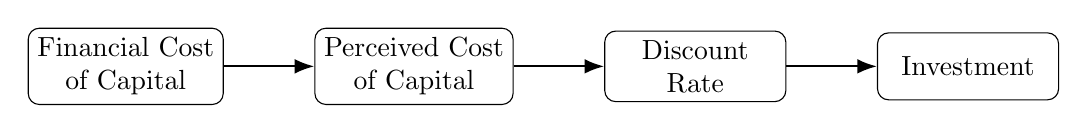
\begin{tikzpicture}[
    processbox/.style={
        draw,
        rounded corners,
        align=center,
        minimum width=2.3cm,
        minimum height=0.85cm
    },
    processarrow/.style={-{Latex[length=2.5mm]}, thick}
]

\node[processbox] (cost) {Financial Cost\\of Capital};
\node[processbox, right=1.15cm of cost]
    (perceived) {Perceived Cost\\of Capital};
\node[processbox, right=1.15cm of perceived]
    (discount) {Discount\\Rate};
\node[processbox, right=1.15cm of discount]
    (investment) {Investment};

\draw[processarrow] (cost) -- (perceived);
\draw[processarrow] (perceived) -- (discount);
\draw[processarrow] (discount) -- (investment);

\end{tikzpicture}
\end{center}



\begin{itemize}
    \item How do firms estimate cost of capital?
    \item How do discount rates vary with perceived cost of capital?
    \item How do discount rates affect investment?
\end{itemize}

% Builds on question from Poterba and Summers (1995): Why are reported discount rates above cost of capital?
% \begin{itemize}
%     \item Gormsen and Huber (2025) looks at changes in gap over time
% \end{itemize}

\end{frame}


\begin{frame}{Innovation}
% Innovation flowchart; yellow denotes novel data and wedge boxes are neutral.
\begin{center}
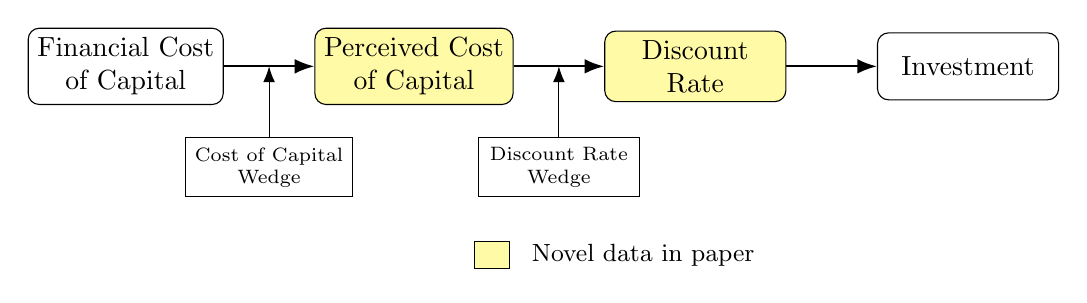
\begin{tikzpicture}[
    processbox/.style={
        draw,
        rounded corners,
        align=center,
        minimum width=2.3cm,
        minimum height=0.85cm
    },
    measured/.style={processbox, fill=yellow!35},
    wedgebox/.style={
        draw,
        align=center,
        minimum width=2.05cm,
        minimum height=0.75cm,
        font=\scriptsize
    },
    processarrow/.style={-{Latex[length=2.5mm]}, thick},
    wedgearrow/.style={-{Latex[length=2mm]}, thin}
]

\node[processbox] (cost) {Financial Cost\\of Capital};
\node[measured, right=1.15cm of cost]
    (perceived) {Perceived Cost\\of Capital};
\node[measured, right=1.15cm of perceived]
    (discount) {Discount\\Rate};
\node[processbox, right=1.15cm of discount]
    (investment) {Investment};

\coordinate (mid1) at ($(cost.east)!0.5!(perceived.west)$);
\coordinate (mid2) at ($(perceived.east)!0.5!(discount.west)$);

\draw[processarrow] (cost) -- (perceived);
\draw[processarrow] (perceived) -- (discount);
\draw[processarrow] (discount) -- (investment);

\node[wedgebox, below=0.9cm of mid1] (costwedge)
    {Cost of Capital\\Wedge};
\node[wedgebox, below=0.9cm of mid2] (discountwedge)
    {Discount Rate\\Wedge};

\draw[wedgearrow] (costwedge.north) -- (mid1);
\draw[wedgearrow] (discountwedge.north) -- (mid2);

\node[
    draw,
    fill=yellow!35,
    minimum width=0.45cm,
    minimum height=0.35cm,
    below=0.55cm of discountwedge,
    xshift=-0.85cm
] (legendbox) {};
\node[
    right=0.15cm of legendbox,
    anchor=west,
    font=\small
] {Novel data in paper};

\end{tikzpicture}
\end{center}


\begin{itemize}
    \item Novel dataset
    \begin{itemize}
        \item Authors hand-collect new data on perceived cost of capital and discount rates
        \item My back-of-the-envelope calculation: at one minute per paragraph, reading transcripts took at least 2,000 hours and conservatively cost \$50,000 in RA wages
    \end{itemize}
    \item Studies time variation in discount rate wedge within firm
    \begin{itemize}
        \item \citet{poterba-summers-1995} survey CEOs and find a discount rate wedge
    \end{itemize}
    \item Characteriziation of chain of transmission
    \begin{itemize}
        \item cost of capital wedge and discount rate wedge
    \end{itemize}
\end{itemize}
\end{frame}

\begin{frame}{Results}
\begin{figure}[ht]
\centering
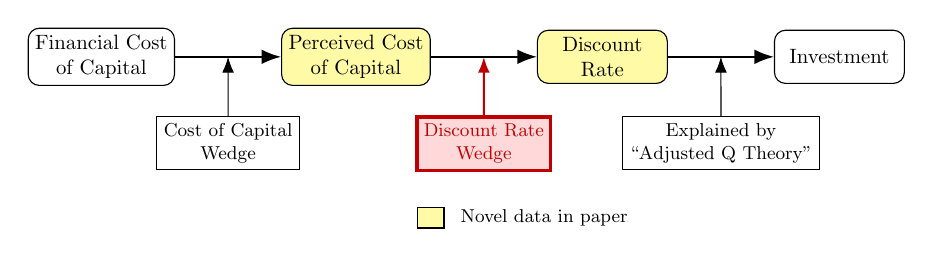
\begin{tikzpicture}[
    scale=0.75,
    transform shape,
    mainbox/.style={
        draw,
        rounded corners,
        align=center,
        minimum width=2.2cm,
        minimum height=0.9cm
    },
    measured/.style={
        mainbox,
        fill=yellow!35
    },
    explanation/.style={
        draw,
        align=center,
        minimum width=1.9cm,
        minimum height=0.9cm,
        font=\small
    },
    wedgebox/.style={
        explanation,
        draw=red!75!black,
        fill=red!15,
        text=red!75!black,
        very thick
    },
    mainarrow/.style={-{Latex[length=2.5mm]}, thick},
    verticalarrow/.style={-{Latex[length=2mm]}, thin}
]

% Main boxes
\node[mainbox] (cost) {Financial Cost\\of Capital};
\node[measured, right=1.8cm of cost]
    (perceived) {Perceived Cost\\of Capital};
\node[measured, right=1.8cm of perceived]
    (discount) {Discount\\Rate};
\node[mainbox, right=1.8cm of discount]
    (investment) {Investment};

% Arrow midpoints
\coordinate (mid1) at ($(cost.east)!0.5!(perceived.west)$);
\coordinate (mid2) at ($(perceived.east)!0.5!(discount.west)$);
\coordinate (mid3) at ($(discount.east)!0.5!(investment.west)$);

% Main arrows
\draw[mainarrow] (cost) -- (perceived);
\draw[mainarrow] (perceived) -- (discount);
\draw[mainarrow] (discount) -- (investment);

% Explanatory boxes
\node[explanation, below=1cm of mid1]
    (measurement) {Cost of Capital\\Wedge};

\node[wedgebox, below=1cm of mid2]
    (wedge) {Discount Rate\\Wedge};

\node[explanation, below=1cm of mid3]
    (theory) {Explained by\\``Adjusted Q Theory''};

% Vertical arrows
\draw[verticalarrow] (measurement.north) -- (mid1);
\draw[
    -{Latex[length=2mm]},
    draw=red!75!black,
    thick
] (wedge.north) -- (mid2);
\draw[verticalarrow] (theory.north) -- (mid3);

% Legend
\node[
    draw,
    fill=yellow!35,
    minimum width=0.45cm,
    minimum height=0.35cm,
    below=0.6cm of wedge,
    xshift=-0.9cm
] (legendbox) {};

\node[
    right=0.15cm of legendbox,
    anchor=west,
    font=\small
] {Novel data in paper};

\end{tikzpicture}
\end{figure}

\footnotesize
\begin{itemize}
    \item Discount rate wedge explains gap between financial cost of capital and investment
    \item Wedge increased by 2.5pp between 2002 and 2021 despite declining perceived cost of capital
    % \item 1pp increase in wedge is associated with 0.8pp decline in investment
    \item Modelling wedge makes sensitivity of investment to changes in financial COC fall by an order of magnitude
\end{itemize}

\begin{alertblock}{Puzzle}
    What drives changes in the discount rate wedge?
\end{alertblock}

\begin{itemize}
    \item Authors show discount rate is sticky, but why?
    \item Higher market power is associated with larger discount rate wedge, but explanatory power is limited
\end{itemize}
\end{frame}

% \begin{frame}{Summary of Results}
% \begin{itemize}
%     \item financial cost of capital predicts perceived cost of capital
%     \item perceived cost of capital have little short and medium term effects on discount rates
%     \item discount rate wedge increased by 2.5pp between 2002 and 2021 despite declining perceived cost of capital
%     \item 1pp increase in discount wedge is associated with 0.8pp drop in investment
%     \item adjusted Q-theory explains most of missing investment
%     \item sensitivity of investment to changes in financial cost of capital fall by an order of magnitude
%     \item firms with high market power have maintained discount rates while increasing discount rate wedges
% \end{itemize}    
% \end{frame}

% \begin{frame}{Data}
%     \begin{itemize}
%         \item Firms that report discount rates in multiple periods account for only 15\% of listed firms in Compustat
%         \begin{itemize}
%             \item They have only 257 observations among firms with at least two reported discount rate wedges
%         \end{itemize}
%         \item 
%     \end{itemize}
% \end{frame}

\begin{frame}{Cost of Capital Wedge}
    \shortflowchart{1}
\end{frame}

\begin{frame}{Cost of Capital Wedge}
    \begin{table}[htbp]
    \centering
    \caption{Perceived and Financial Cost of Capital
    (\(N = 1{,}981\))}
    \label{tab:perceived_financial_coc}
    \begin{tabular}{lcccc}
        \toprule
        Financial cost-of-capital measure
            & Coefficient
            & Standard error
            & Fixed effects
            & Within \(R^2\) \\
        \midrule
        Fin. COC (country level)
            & 0.97
            & (0.14)
            & Country
            & 0.055 \\

        Fin. COC (country level)
            & 0.81
            & (0.20)
            & Firm
            & 0.094 \\

        Fin. COC (firm level)
            & 0.69
            & (0.086)
            & Country
            & 0.094 \\

        Fin. COC (firm level)
            & 0.47
            & (0.13)
            & Firm
            & 0.077 \\
        \bottomrule
    \end{tabular}

    \begin{minipage}{0.92\linewidth}
        \footnotesize
        \vspace{0.5em}
        \textit{Notes:} The dependent variable is the firm's perceived
        cost of capital.
    \end{minipage}
\end{table}

\begin{itemize}
    \item point estimates close to 1
    \begin{itemize}
        \item classical measurement error of financial cost of capital would create downward bias
        % \item assuming 50pp annual return sd, implies 1pp COE measurement error, leading to 
    \end{itemize}
    \item $R^2$ is low
\end{itemize}
\end{frame}

\begin{frame}{Discount Rate Wedge}
    \shortflowchart{2}
\end{frame}

\begin{frame}{Discount Rate Wedge}
    \begin{table}[htbp]
    \centering
    \caption{Discount Rates and the Perceived Cost of Capital}
    \label{tab:discount_rates_perceived_coc}
    \begin{tabular}{lccc}
        \toprule
        & (1) & (2) & (3) \\
        \midrule
        Perceived COC (observed)
            & 0.68 & 0.43 & 0.36 \\
            & (0.093) & (0.12) & (0.092) \\
        \midrule
        Observations
            & 257 & 257 & 257 \\
        Fixed effects
            & Country & Firm & Firm/quarter \\
        $Pr(slope =1)$
            & 0.00086 & 0.000011 & \(1.8e$-$09\) \\
        Within \(R^2\)
            & 0.17 & 0.37 & 0.28 \\
        \bottomrule
    \end{tabular}

    \begin{minipage}{0.85\linewidth}
        \footnotesize
        \vspace{0.5em}
        \textit{Notes:} The dependent variable is the firm's discount
        rate.
    \end{minipage}
\end{table}
    \begin{itemize}
        \item Coefficients much smaller than 1 indicating slow adjustment of discount rate wedge
        \item Stylized model makes exogeneity assumption seem reasonable
    \end{itemize}
\end{frame}

\begin{frame}{Discount Rate Wedge}
    \begin{columns}[c,onlytextwidth]
        \begin{column}{0.49\textwidth}
            \centering
            \includegraphics[width=\linewidth,height=0.76\textheight,keepaspectratio]{figures/discount_rate_wedge.png}
        \end{column}
        \begin{column}{0.49\textwidth}
            \centering
            \includegraphics[width=\linewidth,height=0.76\textheight,keepaspectratio]{figures/discount_rate_wedge_separated.png}
        \end{column}
    \end{columns}
    \begin{itemize}
        \item Change in perceived COC has minimal short-run effect on the discount rate
        \item Discount rate moves more slowly than perceived COC
    \end{itemize}
\end{frame}


\begin{frame}{Discount Rate vs Investment}
    \shortflowchart{3}
\end{frame}

\begin{frame}{Discount Rate vs Investment}
    \begin{footnotesize}
        \footnotesize
        \begin{table}[htbp]
    \centering
    \caption{Investment and Discount Rates}
    \label{tab:investment_discount_rates}
    \begin{tabular}{lcc}
        \toprule
        & (1) & (2) \\
        \midrule
        Discount rate
            & $-0.84$ & \\
            & $(0.23)$ & \\[0.3em]

        Discount rate wedge
            & & $-0.81$ \\
            & & $(0.22)$ \\[0.3em]

        Perceived COC (predicted)
            & & $-1.72$ \\
            & & $(1.16)$ \\
        \midrule
        Observations
            & 1,472 & 1,472 \\
        Fixed effects
            & Firm/quarter & Firm/quarter \\
        Within $R^2$
            & 0.020 & 0.022 \\
        \bottomrule
    \end{tabular}

    \begin{minipage}{0.85\linewidth}
        \footnotesize
        \vspace{0.5em}
        \textit{Notes:} The dependent variable is the annual net investment
        rate measured one year ahead.
    \end{minipage}
\end{table}
    \end{footnotesize}
    \begin{itemize}
        \item Estimates close to negative one (as predicted by model) and remarkably stable
        % \item One endogeneity story: risk premia decreases investment and increases discount rate wedge, leading to more negative coefficient
    \end{itemize}
\end{frame}

\begin{frame}{Discount Rate vs Investment}
    \begin{center}
        \centering
        \includegraphics[width=0.72\linewidth,height=0.66\textheight,keepaspectratio]{figures/adjusted_marginal_q.png}
    \end{center}
Investment behavior consistent with Q theory where firms discount using financial cost of capital plus the cost of capital and discount rate wedges.
\end{frame}


\begin{frame}{Explaining the Discount Rate Wedge}
    \begin{footnotesize}
        \footnotesize
        \begin{table}[htbp]
    \centering
    \caption{Market Power and the Secular Evolution of the Discount-Rate Wedge
    (\(N = 976\))}
    \label{tab:market_power_discount_wedge}
    \begin{tabular}{lccc}
        \toprule
        Independent variable
            & Coefficient
            & Standard error
            & Within \(R^2\) \\
        \midrule
        Market power (2002) $\times$ Year
            & 0.083
            & (0.046)
            & 0.041 \\

        Market power (2002) $\times$ Perceived COC (country mean)
            & $-0.26$
            & (0.12)
            & 0.020 \\

        Market power (2002) $\times$ Perceived COC (firm level)
            & $-0.37$
            & (0.21)
            & 0.078 \\
        \bottomrule
    \end{tabular}

    \begin{minipage}{0.92\linewidth}
        \footnotesize
        \vspace{0.5em}
        \textit{Notes:} The dependent variable is the discount-rate wedge. Specification includes firm fixed effects.
    \end{minipage}
\end{table}
    \end{footnotesize}
\begin{itemize}
    \item Endogeneity concern: higher market power firms are also larger and may have better ability to measure and update estimates of cost of capital
    \item Low $R^2$ with and without firm fixed effects suggests limited explanatory power of market power on discount rate wedge in the timeseries or cross-section 
\end{itemize}
\begin{alertblock}{Puzzle}
    What drives changes in the discount rate wedge?
\end{alertblock}
\begin{itemize}
    \item Why are discount rates sticky?
\end{itemize}
\end{frame}

\begin{frame}{Discussion}
    \begin{itemize}
        \item How much does each wedge drive the gap between investment and Q Theory?
        \begin{itemize}
            \item For example, regress investment gap on cost of capital and discount rate wedge
            \item If firms have better information on perceived cost of capital than is provided by market returns, then COC wedge is not measured correctly
        \end{itemize}
        \vspace{0.3cm}
        \item Why don't firms use more sophisticated discount rate methods?
        \begin{itemize}
            \item Discount rate ignores term structure and assumes project has same distribution of cash flows as firm
            \item Firms that report discount rates in multiple periods account for only 15\% of listed firms assets in Compustat
            \item Firm's discretion around investment opportunities may help explain fixed discount rates
        \end{itemize}
    \end{itemize}
\end{frame}

\appendix

\begin{frame}
    \centering
    \vfill
    {\Huge\bfseries Appendix}
    \vfill
\end{frame}

\begin{frame}{Literature Review}
    \begin{itemize}
        \item \textbf{How the cost of capital and discount rates shape investment}
        \begin{itemize}
            \item \textit{Papers:} \citet{jorgenson-1963}; \citet{tobin-1969}; \citet{hall-2017}
            \item \textit{Contribution:} Links financial prices, perceived cost of capital, discount rates, and investment in one firm-level dataset.
        \end{itemize}

        \vspace{0.25cm}
        \item \textbf{Measuring implied cost of capital}
        \begin{itemize}
            \item \textit{Papers:} \citet{fama-french-1997}; \citet{easton-2004}
            \item \textit{Contribution:} Directly measures firms' perceived cost of capital.
        \end{itemize}

        \vspace{0.25cm}
        \item \textbf{How asset prices affect investment}
        \begin{itemize}
            \item \textit{Papers:} \citet{bond-edmans-goldstein-2012}; \citet{baker-stein-wurgler-2003}
            \item \textit{Contribution:} Argues for a discount-rate channel through which equity prices affect long-run investment without equity issuance.
        \end{itemize}
    \end{itemize}
\end{frame}

\begin{frame}{References}
    \scriptsize
    \nocite{gormsen-huber-2025}
    \bibliographystyle{apalike}
    \bibliography{references}
\end{frame}

\end{document}
